




\section{Algunas identidades}

Una identidad sobre los coeficientes binómicos que es muy útil es la
siguiente.

\begin{proposition}[Simetría en los Coeficientes Binómicos]
  Dados $n, k \in \nset$, se cumple

  $$ {n \choose k} = {n \choose n-k} $$
\end{proposition}

Se podría demostrar mediante su expresión como fracción de factoriales, pero
más elegante sería dar una definición combinatoria. En este caso, es
bastante sencilla.

\begin{proof}
  Recuerde que el coeficiente binómico

  $$ {n \choose k} $$

  \noindent indica las distintas selecciones de $k$ elementos de un conjunto
  de $n$ elementos, sin tener en cuenta el orden. Pero, si se fija, al
  seleccionar $k$ elementos, también está seleccionando los $n-k$ elementos
  restantes. Es decir, los elementos que deshecha es como si también los
  seleccionara, por lo que el número de selecciones posibles sería igual que
  el número de las distintas formas de dechechar elementos.a
\end{proof}

Ahora, vamos a ver otra identidad que es muy útil.

\begin{proposition}[Fórmula de Pascal]
  Dados $k, n \in \nset$ siendo $1 \leq k \leq n-1$. Se cumple

  $$ {n \choose k} = {n-1 \choose k} + {n-1 \choose k-1} $$
\end{proposition}

La justificación de los valores entre los que se pueden mover las variables
que aparecen, lo que debe tener en cuenta es que, en el desarrollo del
coeficiente binómico no aparezca un factorial de un número negativo. Sí
puede aparecer $0!$, que, como dijimos, vale 1.

También hay quien la llama Regla de Pascal o Identidad de Pascal.

Se pueden dar varias demostraciones de este hecho. Una muy directa y
sencilla es mediante manipulaciones algebraicas de esos coeficientes
binómicos. Es bastante fácil. También se puede dar una demostración
combinatoria que es más creativa y entretenida. Sería la siguiente.

\begin{proof}
  Sea $S$ un conjunto de $n$ elementos. Designaremos por $S_k$ al conjunto
  de todos sus subconjuntos de tamaño $k$. Se podría expresar como $S_k =
  \mathcal{P}_k(S)$. Como ya sabemos por combinatoria, se tiene que

  $$ \card(S_k) = {n \choose k} $$

  Lo que pretendemos hacer a continuación será, a partir de la selección de
  un elemento arbitrario $e$ de $S$, formar una partición de $S_k$ en dos
  conjuntos de conjuntos de tamaño $k$ tales que los de uno contengan
  siempre a $e$ y los del otro no lo contengan nunca.

  Partimos de un conjunto

  $$ D = S \setminus \{e\} $$

  \noindent que, como es evidente, tiene por tamaño $n-1$.

  A partir de este, generamos el conjunto $D_k$, formado por todos los
  subconjuntos de $D$ de tamaño $k$. Se tiene, por lo que ya sabemos de
  combinatoria, que

  $$ \card(D_k) = {n-1 \choose k} $$

  \iffalse
  Advierta también que $D_k$ consta de todos los subconjuntos de $S$ de
  tamaño $k$ que no contienen a $e$.
  \fi

  Ahora, en lugar de centrarnos en $D_k$, lo hacemos en $D_{k-1}$, es decir,
  el conjunto de todos los subconjuntos de $D$ de tamaño $k-1$. Este tiene
  por tamaño

  $$ \card(D_{k-1}) = {n-1 \choose k-1} $$

  A partir de este, vamos a generar un conjunto $F_k$ simplemente uniendo
  cada uno de sus elementos, que son conjuntos de tamaño $k-1$, con $\{e\}$.
  Por tanto, los conjuntos que constituyen $F_k$ tienen tamaño $k$.
  Alternativamente, podíamos haber dado la definición en forma simbólica
  siguiente:

  $$ F_k = \left\{M \cup \{e\} \st M \in D_{k-1}\right\} $$

  \noindent El tamaño de $F_k$ será, entonces, el mismo que el de $D_{k-1}$,
  que es

  $$ \card(F_k) = \card(D_{k-1}) = {n-1 \choose k-1} $$

  \iffalse
  Advierta que $F_k$ sería también el conjunto de todos los subconjuntos de
  $S$ de tamaño $k$ que contienen a $e$.
  \fi

  Si se fija, todos pares de conjuntos de $D_k$ y $F_k$ son disjuntos,
  puesto que todos los conjuntos que constituyen a $F_k$ contienen al
  elemento $e$, cosa que no sucede para ninguno de los que constituyen a
  $D_k$. Además, entre ambos, forman todos los subconjuntos posibles de $k$
  elementos de $S$, es decir, $S_k$. Es decir,

  $$ S_k = D_k \cup F_k \quad \text{y} \quad D_k \cap F_k = \emptyset $$

  Debido a esto, $D_k$ y $F_k$ forman una partición de $S_k$, tal y como
  pretendíamos. Por tanto, se tiene que

  $$ \card(S_k) = \card(D_k) + \card(F_k) $$

  \noindent o, lo que es lo mismo,

  $$ {n \choose k} = {n-1 \choose k} + {n-1 \choose k-1} $$
\end{proof}

Si se fija, la fórmula anterior nos sirve como definición recursiva del
coeficiente binómico. TKTK.

De la Identidad de Pascal, se puede deducir una versión ligeramente distinta.

\begin{corollary}
  Dados $k, n \in \nset$ siendo $0 \leq k \leq n$. Se cumple

  $$ {n+1 \choose k} = {n \choose k} + {n \choose k-1} $$
\end{corollary}

Advierta que los valores posibles de $k$ son distintos a los del teorema
anterior.

Se podría deducir de forma directa del teorema anterior simplemente haciendo
un cambio de variable. Otra opción sería hacer una demostración manipulando
las expresiones de los coeficientes binómicos. Vamos a optar por dar esta
última.

\begin{proof}
  -

  \begin{alignat*}{2}
    {n \choose k} + {n \choose k-1}
      &= \frac{n!}{k! (n - k)!} + \frac{n!}{(k-1)! (n - k + 1)!} \\
      &= \frac{n! [(n - k + 1) + k]}{k! (n - k + 1)!} = \frac{n! (n + 1)}{k!
        (n - k + 1)} \\
      &= \frac{(n + 1)!}{k! (n - k + 1)!} = {n+1 \choose k}
  \end{alignat*}
\end{proof}

Me gustaría presentar aquí alguna que otra identidad que no se muestran en
el libro pero que tienen cierta utilidad. Por ejemplo, la de Vandermonde.

\begin{theorem}[Identidad de Vandermonde]
  Dados $m, n, k \in \nset$ siendo $m + n \leq k$. Se cumple

  $$ \sum_{i=0}^k {m \choose i}{n \choose k-i} = {m+n \choose k} $$
\end{theorem}

Al igual que con las otras identidades, se puede demostrar de formas
diversas, pero vamos a tratar de dar una explicación combinatoria.

Lo primero que debe advertir es que, en los coeficientes binómicos que se
multiplican, a la izquierda de la igualdad, abajo se tiene a $i$ y a $k -
i$, cuya suma da $k$, que coincide con la parte inferior del coeficiente
binómico a la derecha de la igualdad.







\section{Triángulo de Pascal}

Lo que vamos a presentar a continuación será simplemente jugar con la
expresión del binomio, dando valores concretos, para ver si podemos intuir
algún patrón por el que podamos llegar a una fórmula para el desarrollo de
este tipo de expresión. Más adelante, daremos rigor a las conclusiones que
saquemos aquí.

Consideremos la expresión $(x + y)^4$. Su desarrollo puede obtenerse
efectuando el producto

$$ (x + y)(x + y)(x + y)(x + y) $$

En el desarrollo de este producto, se van a terminar multiplicando todas las
instancias de todos los elementos $x + y$ entre sí. Se producirán todos los
``cruces''. Por tanto, aparecerán términos $\{x \cdot x, x \cdot y, y \cdot
x, y \cdot y\}$. Pero, si los agrupamos y usamos exponentes, en realidad
todas estas se puede representar por $x^{4-k} y^k$ para algún $k \in \nset$
siendo $0 \leq k \leq 4$. Por ejemplo, el término $x^3 y$ se puede obtener
tomando la $y$ de uno de los factores y la $x$ de cada uno de los 3 factores
restantes. Esto se puede hacer de 4 maneras, y, por lo que ya sabemos de
combinatoria, habrá entonces $C(4, 1)$ términos $x^3 y$, que son las
distintas formas en las que puede aparecer un conjunto con una sola $y$
entre todos los de 4 elementos. Se usan combinaciones porque no importa el
orden pues en esta estructura algebraica se cumple la propiedad conmutativa
del producto.

Análogamente, el coeficiente de $x^2 y^2$ será $C(4, 2)$. Aplicando este
mismo razonamiento para todos los posibles términos del desarrollo del
binomio, tenemos

$$ (x + y)^4 = C(4, 0) x^4 y^0 + C(4, 1) x^3 y^1 + C(4, 2) x^2 y^2 + C(4, 3)
x^1 y^3 + C(4, 4) x^0 y^4 $$

\noindent o, si lo prefiere,

$$ (x + y)^4 = {4 \choose 0} x^4 y^0 + {4 \choose 1} x^3 y^1 + {4 \choose 2}
x^2 y^2 + {4 \choose 3} x^1 y^3 + {4 \choose 4} x^0 y^4 $$

La generalización de este resultado para $(x \pm y)^n$ la veremos a
continuación y se la conoce como el Teorema del Binomio. Pero antes de esto,
debemos demostrar algunas cosas sobre los coeficientes binómicos.

La forma de asignar esos coeficientes puede hacerse mediante el uso de una
figura en forma triangular con coeficientes binómicos en su interior como la
que se representa en la figura \ref{fig-triangulo-pascal-1}. Si calculamos
los valores de esos coeficientes binómicos, tenemos la figura
\ref{fig-triangulo-pascal-2}. Dicha figura recibe el nombre de Triángulo de
Pascal.

\begin{figure}
  \centering
  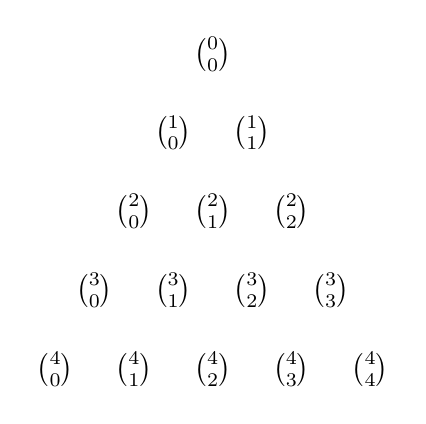
\begin{tikzpicture}
    \foreach \n in {0,...,4} {
      \foreach \k in {0,...,\n} {
        \node at (\k-\n/2,-\n) {${\n \choose \k}$};
      }
      }
  \end{tikzpicture}%
  \label{fig-triangulo-pascal-1}%
  \caption{Triángulo de Pascal}
\end{figure}

\begin{figure}
  \centering
  \begin{tikzpicture}[rotate=-90]
    \foreach \x in {0,1,...,5}
    {
      \foreach \y in {0,...,\x}
      {
        \pgfmathsetmacro\binom{factorial(\x)/(factorial(\y)*factorial(\x-\y))}
        \pgfmathsetmacro\shift{\x/2}
        \node[xshift=-\shift cm] at (\x,\y) {\pgfmathprintnumber\binom};
      }
    }
  \end{tikzpicture}%
  \label{fig-triangulo-pascal-2}%
  \caption{Triángulo de Pascal con los coeficientes calculados}
\end{figure}

Si se fija, el primer y el último elementos en cada fila es un 1. La forma
en que se deduce el valor asignado a una posición es sumando los dos valores
que tiene justo encima. Si se fija, en el fondo lo que hace esto es aplicar
la Identidad de Pascal.





\section{Fórmula del binomio}

Lo normal es llamarlo Teorema del Binomio o Binomio de Newton, pero yo
prefiero llamarlo así.

La principal aplicación del triángulo de Pascal es su aplicación para
desarrollar binomios del tipo $(x + y)^n$.

\begin{theorem}[Fórmula del Binomio]
  Para cada $n \in \nset^{+}$ y para cada par de elementos $x, y \in \rset$,
  se cumple

  $$ (x + y)^n = \sum_{k=0}^n {n \choose k} x^{n-k} y^k $$
\end{theorem}

Este teorema supone la conexión entre la combinatoria y el álgebra.

La siguiente demostración usa el Principio de Inducción. A la gente les
suele gustar más las demostraciones combinatorias. Después de esta, damos
una de este otro tipo.

\begin{proof}
  Haremos la demostración por inducción.

  El caso base sería $n = 1$. En este caso, el resultado es obvio ya que

  $$ x + y = {1 \choose 0} x^{1-0} y^0 + {1 \choose 1} x^{1-1} y^1 = x + y
  $$

  Ahora, vamos con el paso inductivo. Supongamos como hipótesis de inducción
  que se cumple para $n = m$. Habría que comprobar si se cumple también para
  un valor $m+1$.

  \begin{alignat*}{2}
    (x + y)^{m+1}
      &= (x + y)(x + y)^m \\
      &= (x + y)\sum_{k=0}^m {m \choose k}  x^{m-k} y^k \\
      &= \sum_{k=0}^m {m \choose k}  x^{m-k+1} y^k + \sum_{k=0}^m {m \choose
        k}  x^{m-k} y^{k+1} \\
      &= {m \choose 0} x^{m+1} y^0 + {m \choose 1} x^m y^1 + {m \choose 2}
        x^{m-1} y^2 + \cdots + {m \choose m} x^1 y^m + \\
      &+ {m \choose 0} x^m y^1 + {m \choose 1} x^{m-1} y^2 + \cdots + {m
        \choose m-1} x^1 y^m + {m \choose m} x^0 y^{m} \\
  \end{alignat*}

  Observamos que cada término de la forma $x^{m+1-p} y^p$, para $p$ distinto
  de 0 y de $m+1$, aparece dos veces, con coeficientes

  $$ {m \choose p} \quad \text{y} \quad {m \choose p-1} $$

  Aplicando entonces la Identidad de Pascal, se tiene que la suma de esos
  dos coeficientes es

  $$ {m \choose p} + {m \choose p-1} = {m+1 \choose p} $$

  \noindent Por tanto, el desarrollo del binomio queda como

  \begin{alignat*}{2}
    (x + y)^{m+1}
    &= {m+1 \choose 0} x^{m+1} y^0 + {m+1 \choose 1} x^m y^1 + {m+1 \choose
      2} x^{m-1} y^2 + \\
    &+ \cdots + {m+1 \choose m} x^1 y^m + {m+1 \choose m+1} x^0 y^{m+1} \\
    &= \sum_{i=0}^{m+1} {m+1 \choose k} x^{m+1-k} y^k
  \end{alignat*}
\end{proof}

Otra demostración que se podría hacer es una demostración combinatoria.

\begin{proof}
  % https://www.youtube.com/watch?v=Kq7tdEMjrOg

  Vamos a ver varios casos particulares y analizarlos desde el punto de
  vista de la combinatoria.

  Por un lado, tenemos que si $x = y = 1$, se tiene que dar

  $$ (1 + 1)^n = \sum_{k=0}^n {n \choose k} $$

  \noindent Analizándolo desde la combinatoria, podríamos decir que, en la
  parte derecha, cada sumando

  $$ {n \choose k} $$

  \noindent indica el número de subconjuntos de tamaño $k$ que se pueden
  tomar de un conjunto de tamaño $n$. Como para los distintos tamaños, esos
  conjuntos de subconjuntos son disjuntos entre sí, se puede aplicar el
  Principio de la Suma y calcular así el número total de subconjuntos de un
  conjunto de tamaño $n$. Es decir,

  $$ \sum_{k=0}^n {n \choose k} $$

  Por otro lado, podemos calcular el número de subconjuntos de un conjunto
  de tamaño $n$ pensando en permutaciones. Imagínelo como un código binario.
  Tomamos una lista cualquiera de los $n$ elementos y, sobre estos
  elementos, ponemos ceros y unos. Un 0 indica que el elemento que iba en
  esa posición no estará presente en el subconjunto que estamos formando.
  Por el contrario, un 1 indicará que sí lo está. Así, se tienen
  permutaciones con repetición de 2 elementos de orden $n$, es decir,

  $$ PR(2, n) = 2^n = (1 + 1)^n $$

  \noindent que también será, tal y como hemos dicho, el número de
  subconjuntos de un conjunto con $n$ elementos.

  Subimos ahora un ``escalón'' y aumentamos la dificultad. Ahora, queremos
  demostrar que

  $$ (1 + x)^n = \sum_{k=0}^n {n \choose k} x^k $$

  Lo que vamos a contar aquí son el número de aplicaciones con un dominio de
  $n$ elementos y un codominio de $1 + x$ elementos, es decir, el tamaño de
  todas las $G \in \mathcal{F}(n, 1+x)$.

  Es fácil deducir que se tienen $(1 + x)^n$ aplicaciones de ese tipo.
  Simplemente, tiene que pensar que, para el primer elemento del dominio, se
  puede elegir entre $1 + x$ elementos del codominio. Para el segundo,
  también se tienen $1 + x$ posibilidades de imagen, al tener el codominio
  ese número de elementos. Esto mismo no se hacce solo con el primero, sino
  que sucedería con todos, ya que no imponemos ninguna restricción al tipo
  de aplicación (por ejemplo, no se dice que tenga que ser inyectiva). Por
  tanto, aplicando el Principio del Producto, se tiene que existen $(1+x)^n$
  posibles aplicaciones $G \in \mathcal{F}(n, 1+x)$.

  Por otro lado, podemos ir haciendo este mismo razonamiento pero
  particularizado para aplicaciones que tienen $k$ elementos para cada 



















\end{proof}

Como caso particular, se tiene el caso en el que una de esas variables, por
ejemplo, la $y$, valga 1.

\begin{corollary}
  Para cada $n \in \nset^{+}$ y para cada elemento $x \in \rset$, se cumple

  $$ (1 + x)^n = \sum_{k=0}^n {n \choose k} x^k $$
\end{corollary}

Tanto el Teorema del Binomio como este corolario ese $\rset$ se puede
sustituir por cualquier conjunto con una estructura de anillo conmutativo.

Observe también que este teorema nos permite también deducir de forma
inmediata una proposición que se vio en el capítulo anterior

$$ \sum_{k=0}^n C(n, k) = \sum_{k=0}^n {n \choose k} = 2^n $$

Si se da el valor ${-1}$ a la variable en el último corolario, se tiene

$$ 0 = ({-1})^n \sum_{k=0}^k {n \choose k} $$

\begin{theorem}
  Dados $m, k \in \nset$ siendo $k \leq m$. Se cumple

  $$ {m+1 \choose k+1} = {k \choose k} + {k+1 \choose k} + {k+2 \choose k} +
  \cdot + {m-1 \choose k} + {m \choose k} $$
\end{theorem}

\begin{proof}
  La demostración se hará por inducción.

  Sea $S$ el conjunto de los números naturales para los que se satisface la
  igualdad. Veamos que $1 \in S$. En efecto, si $k = 0$, se tiene

  $$ {0 \choose 0} + {1 \choose 1} = 1 + 1 = {2 \choose 1} $$

  \noindent y, si $k = 1$, se tiene

  $$ {1 \choose 1} = 1 = {2 \choose 2} $$

  Así, pues, $1 \in S$. Supongamos que $m \in S$. Entonces, por hipótesis de
  inducción, para todo $k$ tal que $0 \leq k \leq m$, se satisface la
  igualdad

  $$ {m+1 \choose k+1} = {k \choose k} + {k+1 \choose k} + \cdot + {m
  \choose k} $$


  Hay que probar que $m+1 \in S$, es decir, hay que probar que se satisface,
  para todo $k \in \nset$ tal que $0 \leq k \leq m+1$, la igualdad

  $$ {m+2 \choose k+1} = {k \choose k} + {k+1 \choose k} + \cdots + {m+1
  \choose k} $$

  Observamos que el miembro de la derecha es

  $$ {m+1 \choose k+1} + {m+1 \choose k} $$

  \noindent si $0 \leq k \leq m$, ya que $m \in S$. Pero por la Identidad de
  Fermat, se tiene entonces

  $$ {m+2 \choose k+1} $$

  \noindent Si $k = m+1$, la igualdad es trivial. Por tanto, $m+1 \in S$ y
  $S = \nset$.
\end{proof}







\section{Coeficientes multinómicos}

\begin{deffinition}[Coeficiente Multinómico]
  Sean $n, n_1, n_2, n_3, \ldots, n_k \in \nset$ con

  $$ n = \sum_{i=1}^k n_i$$

  \noindent Se define el \emph{coeficiente multinómico} (\emph{multinomial
  coefficient}) $P(n, n_1, n_2, n_3, \ldots, n_k)$ como

  $$ P(n, n_1, n_2, n_3, \ldots, n_k) = \frac{n!}{{n_1}!{n_2}!{n_3}! \cdots
  {n_k}!} $$

  \noindent cosa que también se designará como

  $$ {n \choose {{n_1} {n_2} {n_3} \cdots {n_k}}} $$
\end{deffinition}

\begin{theorem}
  Dados $n$ objetos de $k$ tipos con $n_i$ objetos del tipo $i$, para $1
  \leq i \leq k$ y con

  $$ \sum_{i=1}^k n_i = n $$

  \noindent entonces hay

  $$ {n \choose {{n_1} {n_2} {n_3} \cdots {n_k}}} $$

  \noindent ordenaciones distintas de estos $n$ objetos.

  Consideraremos que dos ordenaciones son iguales si para cada $i$ siendo $1
  \leq i \leq n$ los objetos que ocupan el lugar $i$ son del mismo tipo.
\end{theorem}

Advierta que, aunque sea parecido al coeficiente binómico, sí se tiene en
cuenta el orden en el que se presentan las agrupaciones de elementos
distintos. Dentro de una agrupación de objetos, no importa el orden en el
que se presenten los distintos elementos, pero TKTK.

Si se fija, los coeficientes multinómicos reflejan una situación que sería
una mezcla entre permutaciones y combinaciones ya que, en cierto modo,
importa el orden, pero, en otro cierto modo no. En lo que respecta a las
formas de disponer elementos de un mismo tipo, no importa el orden y serían
como combinaciones. Pero, si se analiza de forma global, el orden en el que
se presenten elementos de tipos diferentes sí se tiene en cuenta para
considerar distintas a dos disposiciones.

\begin{proof}
  Consideremos el primer tipo de objetos, es decir, el caso $i = 1$. Puesto
  que los $n_1$ objetos de este tipo son indistinguibles, no influye el
  orden relativo entre ellos, tal y como ya hemos explicado. Solo
  necesiatamos calcular las formas de disponer esos $n_1$ elementos en un
  conjunto de $n$, es decir, sin importar el orden en el que se presenten
  esos $n_1$ elementos. Esto se calcula, como es evidente, con
  combinaciones:

  $$ {n \choose n_1} $$

  Una vez fijadas las $n_1$ posiciones de los objetos del primer tipo,
  disponemos de $n - n_1$ lugares para los objetos del segundo tipo, $i =
  2$. Por el mismo argumento, tendremos

  $$ {n - n_1 \choose n_2} $$

  \noindent formas de seleccionar los lugares.

  Repitiendo el proceso, llegamos a que los objetos del tipo $k$, es decir,
  el último de los distintos tipos de objetos, tienen que ocupar los $n_k$
  lugares restantes. Como es evidente, solo hay una forma de colocarlos, que
  se reflejaría en la igualdad siguiente:

  $$ {n - (n_1 + n_2 + n_3 + \cdots + n_{k-1}) \choose n_k} = {n_k \choose
  n_k} = 1 $$

  Sobre estas posibilidades podemos aplicar el Principio del Producto.
  Tenemos entonces que el total de disposiciones distintas según estas
  reglas sería

  $$ {n \choose n_1} {n - n_1 \choose n_2} {n - (n_1 + n_2) \choose n_3}
  \cdots {n - (n_1 + n_2 + n_3 + \cdots + n_{k-1}) \choose n_k} $$

  \noindent que, desarrollando los coeficientes binómicos, se convierte en

  $$ \frac{n!}{{n_1}! (n - n_1)!} \cdot \frac{(n - n_1)!}{{n_2}! (n - (n_1 +
  n_2))!} \cdot \frac{(n - (n_1 + n_2))!}{{n_3}! (n - (n_1 + n_2 + n_3))!}
  \cdot \cdots \cdot \frac{(n - (n_1 + n_2 + n_3 + \cdots +
  n_{k-1}))!}{{n_k}! 0!} $$

  \noindent y eliminando los factores comunes en el numerador y el
  denominador, se obtiene finalmente

  $$ \frac{n!}{{n_1}! {n_2}! {n_3}! \cdots {n_k}!} $$
\end{proof}





\section{Fórmula de Leibniz}

Los coeficientes multinómicos surgen, análogamente a lo que sucede con los
binómicos, de la consideración de expresiones algebraicas del tipo

$$ (x_1 + x_2 + x_3 + \cdots + x_k)^n $$

\noindent donde los $x_i$ son elementos de un cuerpo (TKTK) y $n \in \nset$.

Si escribimos

$$ (x_1 + x_2 + x_3 + \cdots + x_k)^n = (x_1 + x_2 + x_3 + \cdots + x_k)(x_1
+ x_2 + x_3 + \cdots + x_k) \cdots (x_1 + x_2 + x_3 + \cdots + x_k) $$

Tras efectuar los productos de la derecha y agrupar los términos semejantes,
tenemos que cada término es de la forma

$$ x_1^{n_1} x_2^{n_2} x_3^{n_3} \cdots x_k^{n_k} $$

\noindent con

$$ n_1 + n_2 + n_3 + \cdots + n_k = n $$

\noindent multiplicado por algún coeficiente. Este coeficiente es el número
de formas distintas de seleccionar $n_1$ factores $x_1$, $n_2$ factores
$x_2$, etc. con

$$ n_1 + n_2 + n_3 + \cdots + n_k = n $$

\noindent Por tanto, el coeficiente es

$$ {n \choose n_1 n_2 n_3 \cdots n_k} $$

\noindent Luego

$$ (x_1 + x_2 + x_3 + \cdots + x_k)^n = \sum_{\substack{n_1, n_2, n_3,
\ldots, n_k = 0 \\ n_1 + n_2 + n_3 + \cdots + n_k = n}}^n {n \choose n_1 n_2
n_3 \cdots n_k} x_1^{n_1} x_2^{n_2} x_3^{n_3} \cdots x_k^{n_k} $$





